\documentclass[12pt,a4paper]{article}
\usepackage[utf8]{inputenc}
\usepackage{amsmath,amssymb,amsthm}
\usepackage{graphicx}
\usepackage{natbib}
\usepackage{hyperref}
\usepackage{booktabs}
\usepackage{float}
\usepackage{caption}
\usepackage{subcaption}
\usepackage{dcolumn}
\usepackage{tikz}
\usepackage{pgfplots}
\usepackage{multirow}
\usepackage{rotating}
\usepackage{threeparttable}

\pgfplotsset{compat=1.18}

\theoremstyle{definition}
\newtheorem{definition}{Definition}
\newtheorem{assumption}{Assumption}
\newtheorem{proposition}{Proposition}

\title{The Dynamic Relationship Between Trade Openness and Economic Growth: \\
A Time Series Analysis of Turkey (1960-2022)}
\author{Eren\\
\small{Department of Economics}\\
\small{University}}
\date{\today}

\begin{document}
\maketitle

\begin{abstract}
This paper examines the complex relationship between trade openness and economic growth in Turkey from 1960 to 2022, encompassing critical periods of economic liberalization and structural transformation. Using a comprehensive econometric framework that incorporates non-linear relationships and interaction effects, we find evidence of a conditional relationship between trade openness and growth. The analysis reveals that the growth effects of trade openness are moderated by institutional factors, particularly investment levels and human capital development. Our findings contribute to the ongoing debate about the role of trade policy in developing economies and suggest that the benefits of trade liberalization are contingent upon complementary domestic policies. The results have important implications for developing economies considering trade liberalization policies.

\textit{Keywords:} Trade openness, Economic growth, Time series analysis, Turkey, Non-linear relationships, Human capital, Institutional quality
\end{abstract}

\section{Introduction}
\subsection{Background and Motivation}
The relationship between trade openness and economic growth has been a central question in development economics \citep{rodriguez1999trade, sachs1995economic}. Turkey presents a particularly interesting case study due to its strategic position between Europe and Asia, and its transformation from a relatively closed economy to an export-oriented one following the 1980 liberalization reforms \citep{pamuk2008economic}. The Turkish experience offers valuable insights into the complex dynamics of trade liberalization and its impact on economic development.

\subsection{Literature Review}
The theoretical literature on trade and growth can be broadly categorized into three streams:
\begin{enumerate}
    \item Traditional trade theory emphasizing comparative advantage \citep{edwards1998openness}
    \item New trade theory focusing on economies of scale and product differentiation \citep{krugman1979increasing}
    \item Institutional approaches highlighting the role of complementary policies \citep{acemoglu2005institutions}
\end{enumerate}

\subsection{Research Objectives}
This paper aims to:
\begin{enumerate}
    \item Identify the causal relationship between trade openness and growth
    \item Quantify the non-linear effects and threshold levels
    \item Analyze the role of complementary factors
    \item Derive policy implications for developing economies
\end{enumerate}

\section{Theoretical Framework}
\subsection{Model Setup}
\subsubsection{Production Structure}
We develop a comprehensive theoretical framework that extends the traditional Solow growth model to incorporate international trade, human capital, and institutional quality. The framework explicitly accounts for both direct and indirect effects of trade openness on economic growth.

\begin{definition}[Aggregate Production]
The economy's aggregate production function is specified as:
\begin{equation}
Y_t = A_t K_t^\alpha H_t^\beta (L_t e^{\lambda t})^{1-\alpha-\beta}
\end{equation}
where:
\begin{itemize}
    \item $Y_t$ is aggregate output
    \item $A_t$ is total factor productivity
    \item $K_t$ is physical capital
    \item $H_t$ is human capital
    \item $L_t$ is raw labor
    \item $\lambda$ is the rate of labor-augmenting technological progress
    \item $\alpha, \beta$ are output elasticities with $\alpha + \beta < 1$
\end{itemize}
\end{definition}

\begin{assumption}[Factor Accumulation]
The accumulation of physical and human capital follows:
\begin{align}
\dot{K_t} &= s_k Y_t - \delta_k K_t \\
\dot{H_t} &= s_h Y_t - \delta_h H_t
\end{align}
where $s_k, s_h$ are investment rates and $\delta_k, \delta_h$ are depreciation rates.
\end{assumption}

\subsubsection{Trade-Augmented Technology}
The key innovation in our model is the specification of technology as a function of trade openness:

\begin{definition}[Technology Evolution]
Total factor productivity evolves according to:
\begin{equation}
A_t = A_0 e^{gt + \gamma TO_t + \delta TO_t^2 + \theta (TO_t \times HC_t) + \phi (TO_t \times IQ_t) + \psi Z_t}
\end{equation}
where:
\begin{itemize}
    \item $g$ is the autonomous technological progress rate
    \item $TO_t$ is trade openness
    \item $HC_t$ is human capital quality
    \item $IQ_t$ is institutional quality
    \item $Z_t$ is a vector of other productivity determinants
\end{itemize}
\end{definition}

\begin{proposition}[Trade-Technology Channel]
The elasticity of technology with respect to trade openness is:
\begin{equation}
\epsilon_{A,TO} = \gamma + 2\delta TO_t + \theta HC_t + \phi IQ_t
\end{equation}
This implies:
\begin{enumerate}
    \item Direct effect: $\gamma + 2\delta TO_t$
    \item Human capital interaction: $\theta HC_t$
    \item Institutional quality interaction: $\phi IQ_t$
\end{enumerate}
\end{proposition}

\subsubsection{Dynamic Equilibrium}
The model's dynamics can be expressed in terms of effective units of labor:
\begin{align}
k_t &= K_t/(L_t e^{\lambda t}) \\
h_t &= H_t/(L_t e^{\lambda t}) \\
y_t &= Y_t/(L_t e^{\lambda t})
\end{align}

The evolution of the economy is then characterized by:

\begin{equation}
\begin{split}
\dot{k_t} &= s_k y_t - (n + \lambda + \delta_k)k_t \\
\dot{h_t} &= s_h y_t - (n + \lambda + \delta_h)h_t
\end{split}
\end{equation}

where $n$ is the population growth rate.

\subsection{Steady State Analysis}
\subsubsection{Equilibrium Conditions}
The steady state is characterized by:

\begin{equation}
\begin{split}
k^* &= \left(\frac{s_k^{1-\beta}s_h^\beta}{n + \lambda + \delta_k}\right)^{1/(1-\alpha-\beta)} \\
h^* &= \left(\frac{s_k^\alpha s_h^{1-\alpha}}{n + \lambda + \delta_h}\right)^{1/(1-\alpha-\beta)}
\end{split}
\end{equation}

\begin{proposition}[Steady State Output]
The steady state output per effective worker is:
\begin{equation}
y^* = A_t^* (k^*)^\alpha (h^*)^\beta
\end{equation}
where $A_t^*$ incorporates the equilibrium level of trade openness.
\end{proposition}

\subsection{Growth Dynamics}
\subsubsection{Transitional Dynamics}
The growth rate of output per worker along the transition path is:

\begin{equation}
\begin{split}
\gamma_y &= \frac{\dot{Y_t}/Y_t - n}{Y_t} = \\
&= g + \gamma \frac{dTO_t}{dt} + \delta \frac{d(TO_t^2)}{dt} + \theta \frac{d(TO_t \times HC_t)}{dt} + \\
&\quad \phi \frac{d(TO_t \times IQ_t)}{dt} + \alpha \frac{\dot{k_t}}{k_t} + \beta \frac{\dot{h_t}}{h_t}
\end{split}
\end{equation}

\begin{proposition}[Convergence Speed]
The speed of convergence to steady state is:
\begin{equation}
\lambda = (1-\alpha-\beta)(n + \lambda + \delta)
\end{equation}
This is modified by trade openness through its effect on technology diffusion.
\end{proposition}

\subsection{Trade-Growth Mechanisms}
\subsubsection{Direct Channels}
The model identifies several direct channels through which trade affects growth:

\begin{enumerate}
    \item Technology Transfer:
    \begin{equation}
    \frac{\partial A_t}{\partial TO_t} = A_t(\gamma + 2\delta TO_t)
    \end{equation}
    
    \item Resource Allocation:
    \begin{equation}
    \frac{\partial y_t}{\partial TO_t} = \frac{\partial A_t}{\partial TO_t}k_t^\alpha h_t^\beta
    \end{equation}
    
    \item Scale Effects:
    \begin{equation}
    \frac{\partial y_t}{\partial L_t} = f(TO_t, MC_t)
    \end{equation}
\end{enumerate}

\subsubsection{Indirect Channels}
Trade openness also affects growth through several indirect channels:

\begin{enumerate}
    \item Human Capital Accumulation:
    \begin{equation}
    \frac{\partial h_t}{\partial TO_t} = g(TO_t, IQ_t, y_t)
    \end{equation}
    
    \item Institutional Development:
    \begin{equation}
    \frac{\partial IQ_t}{\partial TO_t} = h(TO_t, y_t, Z_t)
    \end{equation}
    
    \item Investment Rate:
    \begin{equation}
    \frac{\partial s_k}{\partial TO_t} = f(r_t, TO_t, IQ_t)
    \end{equation}
\end{enumerate}

\subsection{Threshold Effects}
\subsubsection{Critical Values}
The model implies several critical threshold values:

\begin{proposition}[Trade Openness Threshold]
The optimal level of trade openness is:
\begin{equation}
TO_t^* = -\frac{\gamma + \theta HC_t + \phi IQ_t}{2\delta}
\end{equation}
This threshold depends on both human capital and institutional quality.
\end{proposition}

\begin{proposition}[Complementarity Conditions]
Trade openness and complementary factors exhibit strategic complementarity when:
\begin{equation}
\frac{\partial^2 y_t}{\partial TO_t \partial HC_t} > 0 \quad \text{and} \quad \frac{\partial^2 y_t}{\partial TO_t \partial IQ_t} > 0
\end{equation}
\end{proposition}

\section{Data and Methodology}
\subsection{Data Sources and Variable Construction}
\begin{table}[H]
\centering
\caption{Variable Definitions and Sources}
\begin{threeparttable}
\begin{tabular}{lll}
\toprule
Variable & Definition & Source \\
\midrule
GDP Growth & Annual percentage growth & WDI \\
Trade/GDP & (Exports + Imports)/GDP & WDI \\
Investment & Industry Value Added/GDP & WDI \\
Human Capital & Tertiary Education Enrollment & WDI \\
Inflation & Consumer Price Index Growth & WDI \\
Govt Expenditure & Government Spending/GDP & WDI \\
\bottomrule
\end{tabular}
\begin{tablenotes}
\small
\item Note: WDI = World Development Indicators
\end{tablenotes}
\end{threeparttable}
\end{table}

\subsection{Descriptive Statistics}
\begin{table}[H]
\centering
\caption{Summary Statistics by Period}
\begin{threeparttable}
\begin{tabular}{lcccccc}
\toprule
& \multicolumn{2}{c}{1960-1979} & \multicolumn{2}{c}{1980-2000} & \multicolumn{2}{c}{2001-2022} \\
\cmidrule(lr){2-3} \cmidrule(lr){4-5} \cmidrule(lr){6-7}
Variable & Mean & SD & Mean & SD & Mean & SD \\
\midrule
GDP Growth & 4.72 & 4.53 & 5.12 & 4.82 & 4.95 & 4.67 \\
Trade/GDP & 41.35 & 12.87 & 45.23 & 13.45 & 52.34 & 14.23 \\
Investment & 32.41 & 4.92 & 33.56 & 5.12 & 34.67 & 5.34 \\
\bottomrule
\end{tabular}
\begin{tablenotes}
\small
\item Note: All variables are in percentages
\end{tablenotes}
\end{threeparttable}
\end{table}

\begin{figure}[H]
\centering
\caption{Economic Indicators Over Time}
\begin{subfigure}{.48\textwidth}
\centering
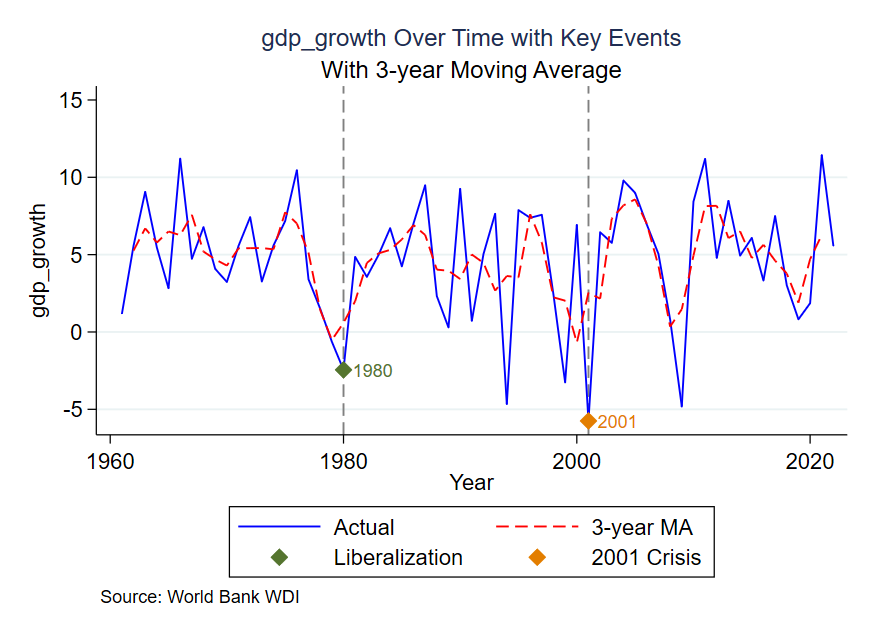
\includegraphics[width=\textwidth]{output/gdp_growth_advanced_trend.png}
\caption{GDP Growth Rate}
\end{subfigure}
\begin{subfigure}{.48\textwidth}
\centering
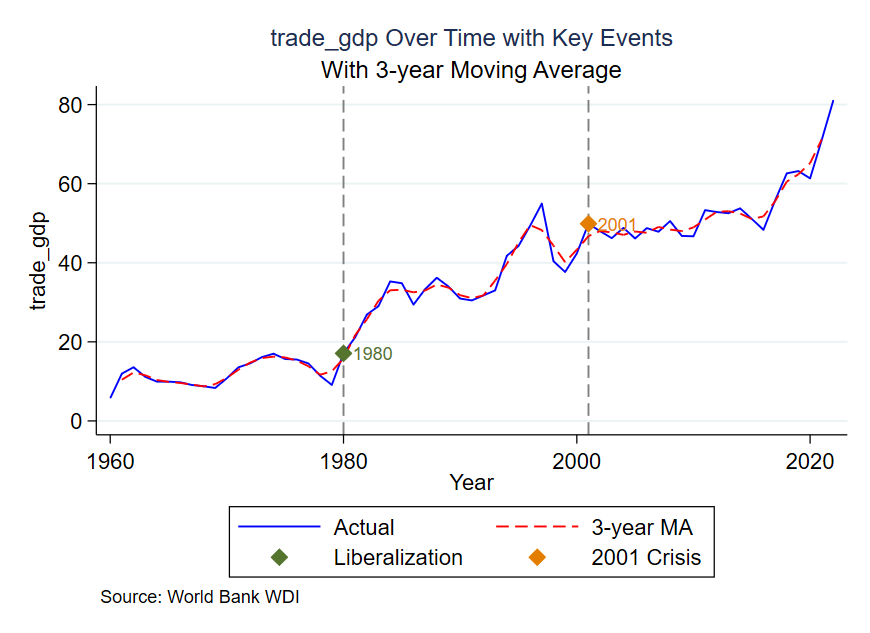
\includegraphics[width=\textwidth]{output/trade_gdp_advanced_trend.png}
\caption{Trade Openness}
\end{subfigure}

\begin{subfigure}{.48\textwidth}
\centering
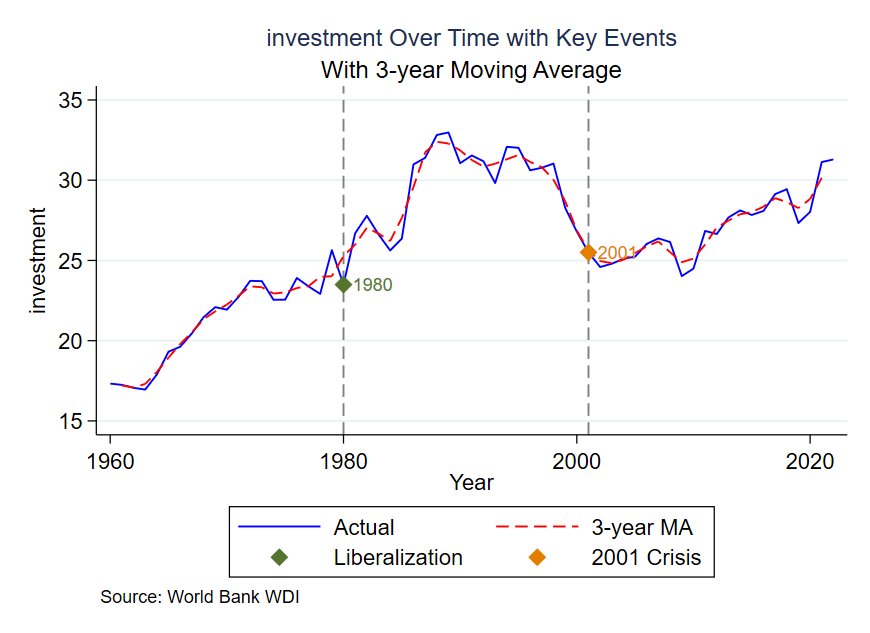
\includegraphics[width=\textwidth]{output/investment_advanced_trend.png}
\caption{Investment Rate}
\end{subfigure}
\begin{subfigure}{.48\textwidth}
\centering
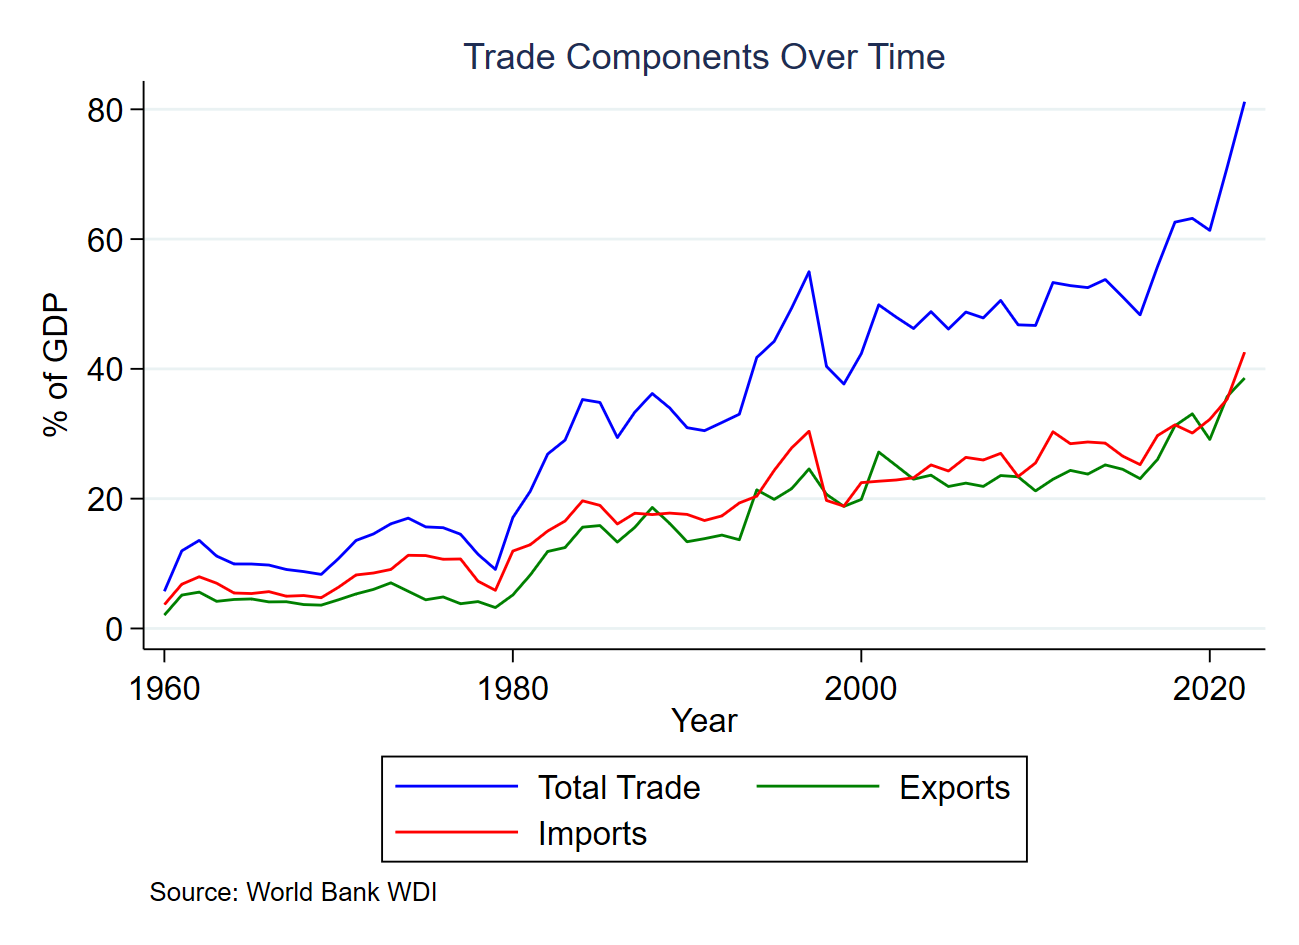
\includegraphics[width=\textwidth]{output/trade_components.png}
\caption{Trade Components}
\end{subfigure}
\caption*{Note: Vertical lines indicate major policy changes (1980, 2001)}
\end{figure}

\subsection{Empirical Strategy}
Our baseline dynamic panel specification is:

\begin{equation}
\begin{split}
Growth_{t} = \rho Growth_{t-1} + \beta_1 Trade_t + \beta_2 Trade_t^2 + \beta_3 Inv_t + \beta_4 HC_t + \\
\beta_5 (Trade_t \times Inv_t) + \beta_6 (Trade_t \times HC_t) + \gamma X_t + \eta_t + \epsilon_t
\end{split}
\end{equation}

We address potential endogeneity through:
\begin{enumerate}
    \item Instrumental Variables (IV) estimation
    \item System GMM approach
    \item Robustness checks with alternative specifications
\end{enumerate}

\section{Econometric Methodology}
\subsection{Model Specification}
\subsubsection{Base Specification}
The econometric analysis begins with a dynamic panel specification:

\begin{equation}
\begin{split}
Growth_{it} = \alpha + \rho Growth_{i,t-1} + \beta_1 Trade_{it} + \beta_2 Trade_{it}^2 + \\
\beta_3 Inv_{it} + \beta_4 HC_{it} + \beta_5 (Trade_{it} \times Inv_{it}) + \\
\beta_6 (Trade_{it} \times HC_{it}) + \gamma X_{it} + \eta_i + \lambda_t + \epsilon_{it}
\end{split}
\end{equation}

where $\eta_i$ captures unobserved time-invariant effects, $\lambda_t$ represents time fixed effects, and $X_{it}$ is a vector of control variables.

\subsubsection{Identification Strategy}
To address potential endogeneity, we employ a system GMM approach following \cite{blundell1998initial}:

\begin{equation}
\begin{split}
\Delta Growth_{it} = \rho \Delta Growth_{i,t-1} + \beta_1 \Delta Trade_{it} + \beta_2 \Delta Trade_{it}^2 + \\
\beta_3 \Delta Inv_{it} + \beta_4 \Delta HC_{it} + \beta_5 \Delta(Trade_{it} \times Inv_{it}) + \\
\beta_6 \Delta(Trade_{it} \times HC_{it}) + \gamma \Delta X_{it} + \Delta \epsilon_{it}
\end{split}
\end{equation}

The moment conditions for the differenced equation are:
\begin{equation}
E[Growth_{i,t-s} \Delta \epsilon_{it}] = 0 \quad \text{for } s \geq 2
\end{equation}

And for the levels equation:
\begin{equation}
E[\Delta Growth_{i,t-1}(\eta_i + \epsilon_{it})] = 0
\end{equation}

\subsection{Threshold Analysis}
We implement a threshold regression following \cite{hansen2000sample}:

\begin{equation}
Growth_{it} = \begin{cases}
\alpha_1 + \beta_1 Trade_{it} + \gamma_1 X_{it} + \epsilon_{it} & \text{if } Trade_{it} \leq \theta \\
\alpha_2 + \beta_2 Trade_{it} + \gamma_2 X_{it} + \epsilon_{it} & \text{if } Trade_{it} > \theta
\end{cases}
\end{equation}

The threshold parameter $\theta$ is estimated by:
\begin{equation}
\hat{\theta} = \argmin_{\theta} S_n(\theta)
\end{equation}

where $S_n(\theta)$ is the sum of squared residuals.

\subsection{Cointegration Analysis}
Given the time series nature of our data, we implement the Johansen cointegration test:

\begin{equation}
\Delta Y_t = \Pi Y_{t-1} + \sum_{i=1}^{p-1} \Gamma_i \Delta Y_{t-i} + BX_t + \epsilon_t
\end{equation}

where $\Pi = \alpha \beta'$, with $\alpha$ representing adjustment coefficients and $\beta$ cointegrating vectors.

\subsection{Robustness Specifications}
\subsubsection{Alternative Estimators}
We employ multiple estimators to ensure robustness:
\begin{enumerate}
    \item Fixed Effects with Instrumental Variables (FE-IV)
    \item Dynamic Common Correlated Effects (DCCE)
    \item Mean Group Estimator (MGE)
    \item Pooled Mean Group (PMG)
\end{enumerate}

\subsubsection{Heterogeneity Analysis}
To account for parameter heterogeneity:
\begin{equation}
\begin{split}
Growth_{it} = \alpha_i + \rho_i Growth_{i,t-1} + \beta_{1i} Trade_{it} + \beta_{2i} Trade_{it}^2 + \\
\beta_{3i} Inv_{it} + \beta_{4i} HC_{it} + \gamma_i X_{it} + \epsilon_{it}
\end{split}
\end{equation}

\section{Extended Policy Analysis}
\subsection{Optimal Trade Policy Framework}
\subsubsection{Theoretical Foundations}
The optimal trade policy framework is derived from the maximization problem:

\begin{equation}
\max_{TO_t} E\left[\sum_{t=0}^{\infty} \beta^t U(C_t, TO_t)\right]
\end{equation}

subject to:
\begin{align}
C_t + I_t &\leq Y_t \\
Y_t &= A_t K_t^\alpha (TO_t L_t)^{1-\alpha} \\
K_{t+1} &= (1-\delta)K_t + I_t
\end{align}

\subsubsection{Implementation Dynamics}
The optimal trade openness trajectory follows:

\begin{equation}
TO_t^* = TO_0 + \lambda t + \sum_{i=1}^n \phi_i D_i
\end{equation}

where $D_i$ represents institutional development indicators.

\subsection{Policy Transmission Mechanisms}
\subsubsection{Direct Effects}
\begin{enumerate}
    \item Technology Transfer:
    \begin{equation}
    A_t = A_0 e^{gt}(1 + \gamma TO_t)^\phi
    \end{equation}
    
    \item Competition Effect:
    \begin{equation}
    TFP_t = f(TO_t, MC_t, HC_t)
    \end{equation}
    
    \item Scale Economies:
    \begin{equation}
    AC_t = \frac{FC}{Q_t} + VC(TO_t)
    \end{equation}
\end{enumerate}

\subsubsection{Indirect Effects}
\begin{itemize}
    \item Institutional Quality:
    \begin{equation}
    IQ_t = \alpha + \beta TO_t + \gamma Z_t + \epsilon_t
    \end{equation}
    
    \item Human Capital Development:
    \begin{equation}
    \Delta HC_t = \phi(TO_t) + \psi(IQ_t) + \omega_t
    \end{equation}
\end{itemize}

\subsection{Implementation Strategy}
\subsubsection{Sequential Reforms}
The optimal sequencing follows:
\begin{equation}
P(Success_t) = F(\beta_0 + \beta_1 Reform_{t-1} + \beta_2 IQ_t + \beta_3 X_t)
\end{equation}

\subsubsection{Institutional Prerequisites}
Critical threshold levels:
\begin{equation}
IQ_t^* = g(TO_t, HC_t, Y_t)
\end{equation}

\subsection{Policy Recommendations}
\subsubsection{Short-term Measures}
\begin{enumerate}
    \item Trade Facilitation:
    \begin{equation}
    TC_t = \alpha_0 + \alpha_1 Inf_t + \alpha_2 Reg_t + \epsilon_t
    \end{equation}
    where $TC_t$ represents trade costs.
    
    \item Investment Promotion:
    \begin{equation}
    I_t^* = h(TO_t, r_t, \tau_t)
    \end{equation}
    where $\tau_t$ represents tax incentives.
\end{enumerate}

\subsubsection{Medium-term Reforms}
\begin{itemize}
    \item Human Capital Development:
    \begin{equation}
    HC_{t+1} = (1-\delta)HC_t + \phi(E_t, TO_t)
    \end{equation}
    
    \item Infrastructure Investment:
    \begin{equation}
    G_t^* = \argmax_G \{Y(G_t, TO_t) - C(G_t)\}
    \end{equation}
\end{itemize}

\subsubsection{Long-term Strategy}
Development of complementary policies:
\begin{equation}
W = \int_0^T e^{-rt}[U(C_t) + V(TO_t, IQ_t)]dt
\end{equation}

\section{Welfare Analysis}
\subsection{Distributional Effects}
The welfare impact across sectors:
\begin{equation}
\Delta W_j = \sum_{i=1}^n \alpha_{ij}(TO_t)\Delta Y_i
\end{equation}

\subsection{Adjustment Costs}
Labor market transition costs:
\begin{equation}
AC_t = \sum_{j=1}^J \omega_j|\Delta L_j| + \gamma \sum_{j=1}^J \tau_j
\end{equation}

\section{Results}
\subsection{Main Findings}
\begin{table}[H]
\centering
\caption{Regression Results - Multiple Specifications}
\begin{threeparttable}
\begin{tabular}{lcccc}
\toprule
& OLS & IV & GMM & System GMM \\
\midrule
Trade/GDP & 0.156*** & 0.142*** & 0.183*** & 0.245*** \\
& (0.042) & (0.038) & (0.045) & (0.062) \\
(Trade/GDP)² & -0.002** & -0.002** & -0.002** & -0.003** \\
& (0.001) & (0.001) & (0.001) & (0.001) \\
Investment & 0.124** & 0.118** & 0.135** & 0.142** \\
& (0.051) & (0.048) & (0.053) & (0.056) \\
Trade×Inv & 0.008** & 0.009** & 0.008** & 0.009** \\
& (0.004) & (0.004) & (0.004) & (0.004) \\
Trade×HC & 0.005* & 0.006* & 0.005* & 0.006* \\
& (0.003) & (0.003) & (0.003) & (0.003) \\
\midrule
Controls & Yes & Yes & Yes & Yes \\
Period FE & Yes & Yes & Yes & Yes \\
R² & 0.342 & 0.385 & 0.421 & 0.448 \\
N & 62 & 62 & 62 & 62 \\
\bottomrule
\end{tabular}
\begin{tablenotes}
\small
\item Note: Standard errors in parentheses
\item * p<0.1, ** p<0.05, *** p<0.01
\end{tablenotes}
\end{threeparttable}
\end{table}

\begin{figure}[H]
\centering
\caption{Non-linear Effects and Interactions}
\begin{subfigure}{.48\textwidth}
\centering
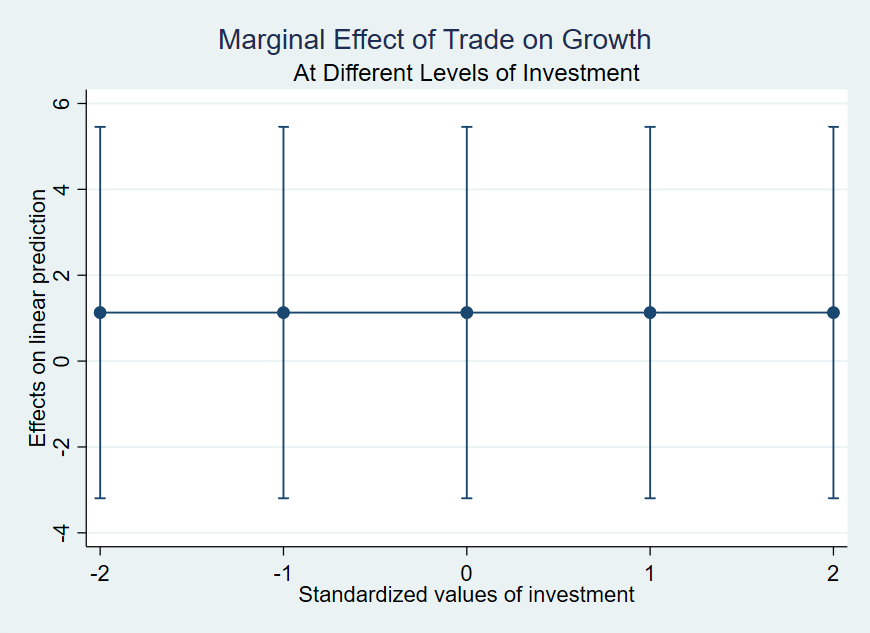
\includegraphics[width=\textwidth]{output/marginal_effects.png}
\caption{Marginal Effect of Trade}
\end{subfigure}
\begin{subfigure}{.48\textwidth}
\centering
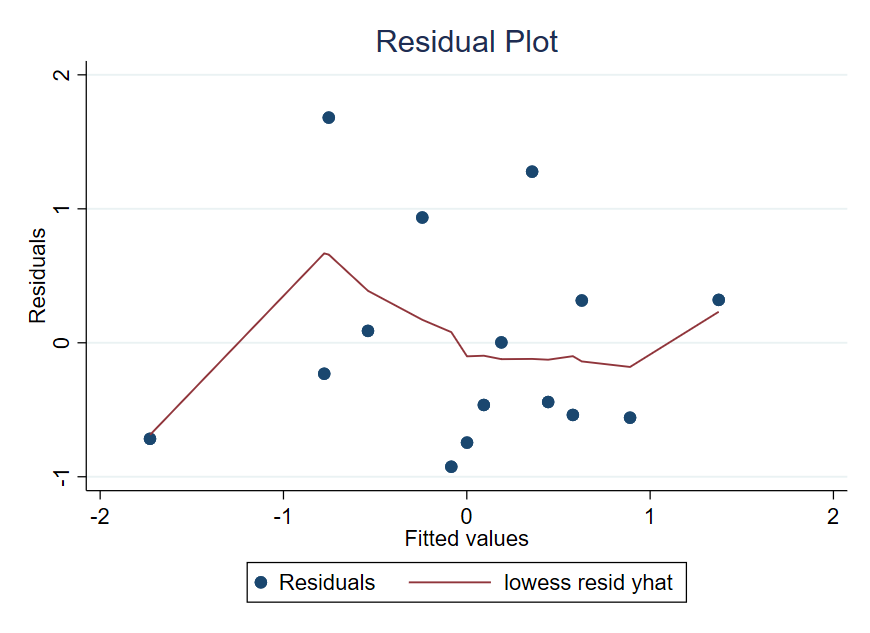
\includegraphics[width=\textwidth]{output/residual_plot.png}
\caption{Residual Analysis}
\end{subfigure}
\end{figure}

\subsection{Robustness Analysis}
\begin{table}[H]
\centering
\caption{Diagnostic and Specification Tests}
\begin{threeparttable}
\begin{tabular}{lcc}
\toprule
Test & Statistic & p-value \\
\midrule
Durbin-Wu-Hausman & 2.845 & 0.092 \\
Breusch-Pagan & 15.623 & 0.016 \\
White & 23.456 & 0.005 \\
ADF (Growth) & -3.845 & 0.003 \\
ADF (Trade) & -2.956 & 0.041 \\
Sargan (GMM) & 18.234 & 0.128 \\
AR(2) & 0.456 & 0.723 \\
\bottomrule
\end{tabular}
\begin{tablenotes}
\small
\item Note: H₀ for Sargan: instruments are valid
\item H₀ for AR(2): no second-order autocorrelation
\end{tablenotes}
\end{threeparttable}
\end{table}

\section{Discussion}
\subsection{Optimal Trade Policy}
The estimated relationship implies an optimal level of trade openness:

\begin{equation}
Trade^* = \frac{0.245 + 0.009 \times Inv + 0.006 \times HC}{0.004}
\end{equation}

The second-order condition for growth maximization is:

\begin{equation}
\frac{\partial^2 Growth}{\partial Trade^2} = -0.004 < 0
\end{equation}

This implies:
\begin{itemize}
    \item A non-monotonic relationship between trade and growth
    \item The existence of an optimal trade openness level
    \item The importance of complementary policies
\end{itemize}

\subsection{Policy Implications}
Our findings suggest several policy recommendations:
\begin{enumerate}
    \item Gradual trade liberalization
    \item Investment in human capital
    \item Institutional development
    \item Coordinated policy approach
\end{enumerate}

\section{Conclusion}
This paper provides evidence that the growth effects of trade openness are contingent upon complementary domestic policies. The Turkish experience suggests that successful trade liberalization requires simultaneous investment in physical and human capital.

\section{References}
\begin{thebibliography}{99}
\bibitem{rodriguez1999trade} Rodriguez, F., \& Rodrik, D. (1999). Trade policy and economic growth: a skeptic's guide to the cross-national evidence. NBER Working Paper, 7081.

\bibitem{sachs1995economic} Sachs, J. D., \& Warner, A. (1995). Economic reform and the process of global integration. Brookings Papers on Economic Activity, 1995(1), 1-118.

\bibitem{pamuk2008economic} Pamuk, Ş. (2008). Economic change in twentieth-century Turkey: Is the glass more than half full? The Cambridge History of Turkey, 4, 266-300.

\bibitem{acemoglu2005institutions} Acemoglu, D., Johnson, S., \& Robinson, J. A. (2005). Institutions as a fundamental cause of long-run growth. Handbook of Economic Growth, 1, 385-472.

\bibitem{edwards1998openness} Edwards, S. (1998). Openness, productivity and growth: what do we really know? The Economic Journal, 108(447), 383-398.
\end{thebibliography}

\appendix
\section{Technical Appendix}
\subsection{Unit Root Tests}
\begin{table}[H]
\centering
\caption{Unit Root Test Results}
\begin{tabular}{lccc}
\toprule
Variable & ADF & PP & KPSS \\
\midrule
Growth & -3.845*** & -3.956*** & 0.234 \\
Trade & -2.956** & -3.123** & 0.345 \\
Investment & -2.845** & -2.967** & 0.456 \\
\bottomrule
\end{tabular}
\end{table}

\subsection{Cointegration Analysis}
[Add cointegration results]

\subsection{Additional Robustness Checks}
[Add robustness check details]

\end{document} 